\documentclass[12pt]{scrartcl}
\usepackage{graphicx}
\usepackage{amsmath}

\newcommand{\RN}[1]{%
  \textup{\uppercase\expandafter{\romannumeral#1}}%
}

\begin{document}
\title{Interaction of a "cold plume" with a subduction zone}
\subtitle{Semester Thesis}
\author{Florian Frei}

\maketitle

\newpage

\tableofcontents

\newpage

\section{Motivation}
Seismological measurements from Columbia shown in figure \ref{fig:seism_data} suggests that an rare geological scenario is happening. The geophysical community agrees that what is probably happening is the rare case where a "cold plume" is detached from the lithosphere and interacts with the subduction plate beneath it. In this project the goal is to use a simplified subduction model to simulate what longterm tendencies could develop and investigate the sensitivity on the parameters for the individual scenarios.
\begin{figure}
\includegraphics[scale=0.45]{deep_anomaly_hor_ver.png}
\label{fig:seism_data}
\end{figure}

\section{Geophysical Model}
The skill how to correctly model geophysics for a numerical simulation is to vast that it could fit into a single book much less into a simple report. A good starting point which is essential to understand this project is the book "Introduction to Numerical Geodynamic Modelling" \cite{gerya2009introduction} written by Taras Gerya. This project can also be seen as an additional example in application of geophysical numerical modeling.
\subsection{Physical Equations}
For completeness all equations used in the simulation are listed below. Most equations originate from the fact that the material is seen as a continuum. Therefore one can intuitively guess that the three conservation laws are used for describing its behavior. Namely the conservation of mass, momenta and energy or in this case heat. First the conservation of mass is described by the continuity equation written in Eulerian form as:
\begin{align}
\frac{d \rho}{d t} + \nabla \cdot (\rho \mathbf{v})&=0
\intertext{, and in the Lagrangian form as:}
\frac{D \rho}{D t} + \rho \nabla \cdot \mathbf{v}&=0
\end{align}
, where $\rho$ is the local density of the material and $\mathbf{v}=\begin{pmatrix}v_x\\v_y \end{pmatrix}$ the local velocity.\\
The second law, conservation of momenta, is described by the Navier-Stokes equations. Since this project is a model in two dimensions the reduced Naver-Stokes equation in Eulerian form is written as:
\begin{align}
\frac{\partial \sigma_{xx}'}{\partial x}+\frac{\partial \sigma_{xy}}{\partial y}-\frac{\partial P}{\partial x}+\rho g_x&=\rho \left( \frac{\partial v_x}{\partial t}+v_x\frac{\partial v_x}{\partial x}+v_y\frac{\partial v_x}{\partial y} \right)\\
\frac{\partial \sigma_{yy}'}{\partial x}+\frac{\partial \sigma_{yx}}{\partial y}-\frac{\partial P}{\partial y}+\rho g_y&=\rho \left( \frac{\partial v_y}{\partial t}+v_x\frac{\partial v_y}{\partial x}+v_y\frac{\partial v_y}{\partial y} \right)\\
\intertext{and in Lagrangian form as:}
\frac{\partial \sigma_{xx}'}{\partial x}+\frac{\partial \sigma_{xy}}{\partial y}-\frac{\partial P}{\partial x}+\rho g_x&=\rho \frac{D v_x}{D t}\\
\frac{\partial \sigma_{yy}'}{\partial x}+\frac{\partial \sigma_{yx}}{\partial y}-\frac{\partial P}{\partial y}+\rho g_y&=\rho \frac{D v_y}{D t}\\
\end{align}
Last but not least the third conservation law, conservation of heat, also known as temperature equation, can be derived from Fourier's law of heat conduction and has the following Lagrangian form, assuming $k$ is constant:
\begin{align}
\rho C_p \frac{D T}{D t} &= k (\frac{\partial^2 T}{\partial x^2}+\frac{\partial^2 T}{\partial y^2})+H_r+H_s+H_a+H_L\\
\intertext{or in Eulerian form:}
\rho C_p (\frac{\partial T}{\partial t}+v_x \frac{\partial T}{\partial x} + v_y \frac{\partial T}{\partial y})&= k (\frac{\partial^2 T}{\partial x^2}+\frac{\partial^2 T}{\partial y^2})+H_r+H_s+H_a+H_L
\intertext{In this project only two heating terms are considered relevant namely the adiabatic heating $H_a$ and the shear heating $H_s$. These two are approximated with the following relations:}
H_a &\approx \alpha\cdot T \cdot v_y \cdot \rho \cdot g_y\\
H_s &\approx \sigma_{xx}\cdot \dot{\epsilon}_{xx} + \sigma_{xy}\cdot \dot{\epsilon}_{xy};
\end{align}
All these equations have in common namely that they are all partial differential equations in space and time where mostly an analytical solution cannot be found. Furthermore to find a solution on a domain one requires additional information such as the initial state and boundary conditions. \\
With these tree equation one can depict how the continuum moves and how the temperature develops but what is still missing is the behavior of the material under these changes. This is defined in the rheology of rocks. There are a lot of possible choices for the behavior like visco-elastic, visco-plastic etc. to name just a few. In this project for simplicity we use a well-known empirical rheological relationship \ref{eq:emprheolrel} between strain-rate and differential stress which is of the following form:
\begin{equation}
\dot{\gamma}=A_D h^m (\sigma_d)^n\exp\left( -\frac{E_a+V_a P}{RT} \right)
\label{eq:emprheolrel}
\end{equation}
Note however that $A_D,h,E_a$ and $V_a$ are still parameters which have to be defined. A sensible choice will be shown in section \ref{seq:modelsetup} about the model setup. Finally the property for isotropic, incompressible materials \ref{eq:iim} will also be utilized in this context to describe the rheology.
\begin{equation}
\sigma_{\RN{2}} = 2 \eta_{eff}\dot{\epsilon}_{\RN{2}}
\label{eq:iim}
\end{equation}

\section{Model setup}
\label{seq:modelsetup}
First of all the model setup for a subduction zone will be shown as a basis. This model is utilized for simulating the subduction of a slab from the lithosphere into the asthenosphere. Depending on the properties of the necking area different scenarios occur. The actual model of this project takes a segment of this model and places a "cold plume" above the slab. In this model the interest lies not in the process of breaking of the slab but in the interaction between the slab and the plume where different tendencies develop.
\subsection{Model of a subduction zone}
\begin{figure}[!ht]
\includegraphics[scale=0.6]{subduction_model.pdf}
\caption{model structure of subduction zone}
\end{figure}


\subsection{Segment of this model}




\section{Implementation}

flow diagram
\section{Results}
\section{Conclusion}

\nocite{vargas2013tearing}
\nocite{gerya2009introduction}




\newpage

\bibliographystyle{plain}
\bibliography{references}


\end{document}

